\documentclass[11pt]{article}
\usepackage{latexsym}
\usepackage{amsmath}
\usepackage{listings}[language=Python]
\usepackage{amssymb}
\usepackage{amsthm}
\usepackage{pifont}% http://ctan.org/pkg/pifont
\newcommand{\xmark}{\text{\ding{55}}}
\newcommand{\cmark}{\text{\ding{51}}}

\usepackage{epsfig}
\usepackage[tight]{subfigure}



\DeclareMathOperator*{\minimize}{min}
\DeclareMathOperator*{\maximize}{max}
\newcommand{\HH}{\mathcal{H}}
\newcommand{\X}{\mathcal{X}}
\newcommand{\Y}{\mathcal{Y}}
\newcommand{\V}{\mathbf{V}}

\newcommand{\bs}[1]{\boldsymbol{#1}}

\usepackage{algorithm}
 %on linux you may need to run sudo apt-get install texlive-full to install algorithm.sys
\usepackage{algorithmic}

\usepackage{verbatim}

\newcommand{\handout}[5]{
  \noindent
  \begin{center}
  \framebox{
    \vbox{
      \hbox to 5.78in { {#1} \hfill #2 }
      \vspace{4mm}
      \hbox to 5.78in { {\Large \hfill #5  \hfill} }
      \vspace{2mm}
      \hbox to 5.78in { {\em #3 \hfill #4} }
    }
  }
  \end{center}
  \vspace*{4mm}
}

\newcommand{\lecture}[5]{\handout{#1}{#2}{#3}{#4}{#5}}
\newcommand{\collision}[0]{\mathrm{collision}}
\newcommand{\nocollision}[0]{\overline{\collision}}
\newcommand*{\QED}{\hfill\ensuremath{\square}}

\newtheorem{theorem}{Theorem}
\newtheorem{corollary}[theorem]{Corollary}
\newtheorem{lemma}[theorem]{Lemma}
\newtheorem{observation}[theorem]{Observation}
\newtheorem{proposition}[theorem]{Proposition}
\newtheorem{definition}[theorem]{Definition}
\newtheorem{claim}[theorem]{Claim}
\newtheorem{fact}[theorem]{Fact}
\newtheorem{assumption}[theorem]{Assumption}
\newtheorem{note}[theorem]{Note}

% 1-inch margins, from fullpage.sty by H.Partl, Version 2, Dec. 15, 1988.
\topmargin 0pt
\advance \topmargin by -\headheight
\advance \topmargin by -\headsep
\textheight 8.9in
\oddsidemargin 0pt
\evensidemargin \oddsidemargin
\marginparwidth 0.5in
\textwidth 6.5in

\parindent 0in
\parskip 1.5ex
%\renewcommand{\baselinestretch}{1.25}

\begin{document}

\lecture{Statistical Techniques in Robotics (16-831, S20)}{Lecture \#15
  (Wednesday, February 8)}{Lecturer: Kris Kitani}{Scribes: Zhengyi Luo, Erica Weng}{MDP, Bellman Equations, Value Function}
\
%This section serves as a review of the previous lecture and any other context required to frame the content of the current lecture. 

%You may format the scribes in any way you like, aside from changing font style, size and page format. Please use subsections and paragraphs to increase the readability of your notes.

%Length requirement 1-2 pages.

\section{Recap}
In the previous lectures, we have been focusing on a series of online learning problems that are one-shot: each timestep of the experiment is independent and is not affected by the history or the future state/action of the environment. In this lecture, we will remove this assumption and study \textbf{sequential} learning problems where each action will affect the state of the environment and in turn affect the future state interaction between the agent and the environment. An example application is that of autonomous vehicle control. Given a sequence of car state readings, the goal is to control the car to achieve the maximum reward (or equivalently, the lowest cost) -- that is, not crashing into obstacles and getting to the destination.

\section{Reinforcement Learning}
\begin{table}[h!]
    \centering
    \begin{tabular}{|p{.45\linewidth}|p{.45\linewidth}|}
        \hline $\text { Supervised Learning }$ &  $\text { Reinforcement Learning }$ \\
        \hline  samples given by environment & samples $(x, a)$ drawn through interaction with an environment, which behaves according to certain rules \\ 
        
        samples $(\zeta, R)$ are assumed to be independently and identically distributed & samples within a ``trajectory" $\zeta$ affect the next state (and thus the other relevant values in the next sample, such as reward $R$) \\
        $x, a \sim \mathcal{D} (x,a) $ & $\zeta, R \sim \mathcal{D}(\zeta, R)$ \\
        dataset is composed of $N$ i.i.d datapoints: $\{ (x_1, a_1), (x_2, a_2), \dots, (x_N, a_N) \}$  &     dataset is composed of $N$ trajectory - reward pairs: $\{ (\zeta_1, R_1), (\zeta_2, R_2), \dots, (\zeta_N, R_N) \}$ where $\zeta_i = \{ (x_1, a_1), (x_2, a_2), \dots, (x_T, a_T) \}$ \\
        \hline
    \end{tabular}
    \caption{Comparison of Supervised Learning vs. Reinforcement Learning \cite{slides, littman2015reinforcement,sutton }}
    \label{tab:2}
\end{table}


\begin{table}[h!]
    \centering
    \begin{tabular}{|c|c|c|c|}
        \hline $\text { Problem }$ &  $\text { Sampled }$ & $\text { Evaluative }$ & $\text { Sequential }$ \\
        \hline $\text { PWEA }$ &     $\xmark$ & $\xmark$ & $\xmark$ \\
        \hline $\text { OLC }$ &      $\cmark$ & $\xmark$ & $\xmark$ \\
        \hline $\text { MAB }$ &      $\xmark$ &        $\cmark$ & $\xmark$ \\
        \hline $\text { C-MAB }$ &    $\cmark$ & $\cmark$ & $\xmark$ \\
        \hline $\text { RL }$ &      $\cmark$ & $\cmark$ & $\cmark$ \\
        \hline
    \end{tabular}
    \caption{Setup of the different problems we have learned so far}
    \label{tab:my_label}
\end{table}
Reinforcement learning is a sampled problem because it's impossible to see the entire state space, and thus trajectories (data points) must be sampled. It's an evaluative problem in that we get qualitative feedback, but no information about optimality. And finally, it's a sequential problem, because the order we receive samples matters (within a trajectory), as they depend on each other across time.

\section{Markov Decision Process}
A Markov decision process is a discrete-time stochastic control process. \cite{sutton} It can usually be described by a 4 tuple $\left(S, A, P_{a}, R_{a}\right)$ where:
\begin{itemize}
    \item $S$ is a set of all possible states of the current environment ,
    \item $A$ is a set of all possible actions of the current environment,
    \item $P_a(s_{t+1}|s_t, a_t)$ is the transition dynamics of the environment, and describes the probability that action $a_t$ in state $s_t$ will lead to $s_{t+1}$,
    \item $R_a(s_t)$ or $R_a(s_t, a_t)$ or $R_a(s_t, a_t, s_{t+1})$ is the immediate reward recevied from the environment at time step $t$. 
\end{itemize}

Other relevant definitions of the Markov decision process are: 

\begin{itemize}
    \item $\pi(a_t|s_t)$ is the policy that describes the probability of taking action $a_t$ based on the current state $s_t$. 
    \item $p_0(s_0)$ is the initial state probability, which describes the probability of the environment being initialized to state $s_0$. 
    \item $\gamma$ is the discount factor used to calculate the present value of the future reward.
\end{itemize}

The key assumption of a Markov decision process is the ``Markov Property", which is defined as: 

\textbf{Markov Property:} a state is Markov if and only if
$$P\left[S_{t+1} \mid S_{t}\right]=P\left[S_{t+1} \mid S_{1}, \ldots, S_{t}\right].$$

The above property states that a Markov decision process is ``memory-less", where given the current state, the future state is independent of the past state. Namely, ``the future is independent of the past given the present".  Another way of stating this property is: the state $S_t$ captures all relevant information from the history and can fully describe the current environment. Combining with the transition dynamics $P_a$, a policy $\pi$, and the Markov property, the joint probability of a Markov Decision Process $p\left(s_{0}, \cdots, s_{T}, a_{0}, \cdots, a_{T}\right)$ can be factorized as:

$$p\left(s_{0}, \cdots, s_{T}, a_{0}, \cdots, a_{T}\right)=p_{0}\left(s_{0}\right) \prod_{\text {t = 0 }}^{T-1} P_a\left(s_{t+1} \mid s_{t}, a_{t}\right) \pi\left(a_{t} \mid s_{t}\right).$$


\subsection{Example: Grid World}
\begin{center}
    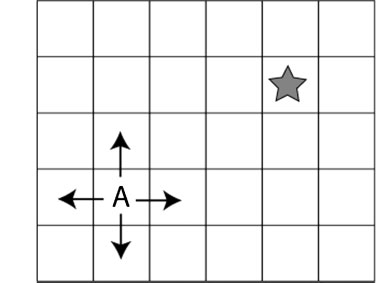
\includegraphics[width=0.5\linewidth]{lec15/grid.png}    
\end{center}

One of the simplest forms of a MDP is navigating in a grid world. Consider the above grid, where each square in the grid represents a state $S$; at each state, you can perform action $a$ to move (up, down, left right). A policy $\pi(a_t|s_t)$ can be defined to take actions based on the current state, a reward $r(s_t)$ can be defined to map a state (block) to a real value, and a transition dynamics $P_a(s_{t+1} | s_t, a_t)$ describes the probability of transition to another state. The policy, reward, and transition dynamics can be either stochastic or deterministic. 




\section{Value Function}
As mentioned before, the key difference between RL and online learning is the need to model \textbf{the future}. RL often models the future in the form of a value function. A value function estimates the total expected return of a trajectory. There are two major forms of value function: state value function $V(s_t)$ which models the total expected return of a trajectory starting in state $s_t$, and a action value function $Q(s_t, a_t)$ which models the total expected return of a trajectory starting in state $s_t$ and performing action $a_t$. Since an expected trajectory needs to be defined with respect to a policy, we often denote the value functions as $V^\pi$ and $Q^\pi$. 


\subsection{State Value Function}
The state value function can be written out as:
$$V^{\pi}(s_t)=\mathbb{E}_{p}\left[r_{t}+r_{t+1}+r_{t+2}+\cdots \mid s_{0}=s_t\right], $$

where the the expectation $\mathbb E_p$ is taken over the policy $\pi$ and the transition dynamics $P_a$. The reward  is defined as $r_{t} \triangleq r\left(s_{t+1}, a_{t}, s_{t}\right) $. The value function can be defined with respect to different time horizons, with:
$$ \text{Infinite horizon return : } V^{\pi}(s_t)=\mathbb{E}_{p}\left[r_{t}+r_{t+1}+r_{t+2}+\cdots \mid s_{0}=s_t\right],$$
$$ \text{Finite horizon return: } V^{\pi}(s_t)=\mathbb{E}_{p}\left[r_{t}+r_{t+1}+r_{t+2}+\cdots r_{T} \mid s_{0}=s_t\right],$$
$$ \text{Infinite horizon: } V^{\pi}(s_t)=\mathbb{E}_{p}\left[\gamma^{0} r_{t}+\gamma^{1} r_{t+1}+\gamma^{2} r_{t+2}+\cdots \mid s_{0}=s_t\right].$$



\subsection{State-Action Value Function}
The state-action value function defines the total expected return of a trajectory starting in the state $s_t$ and taking action $a_t$:

$$Q^{\pi}(s_t, a_t)=\mathbb{E}_{p}\left[\gamma^{0} r\left(s_{t}\right)+\gamma^{1} r\left(s_{1}\right)+\gamma^{2} r\left(s_{2}\right)+\cdots \mid s_{0}=s_t, a_{0}=a_t\right].$$

Intuitively, the state-action value function, or ``Q function" measures the future return based on taking the action $a_t$ at state $s_t$. 

Based on the definition of $V^\pi$ and $Q^\pi$, we have the following relationship: 

$$V^{\pi}(s_t)=\sum_{a_t} \pi(a_t \mid s_t) Q^{\pi}(s_t, a_t)$$
% $$Q^{\pi}(s_t, a_t)= \sum_{s_{t+1}}P_a(s_{t+1}|s_t, a_t)[r(s_t, a_t, s_{t+1}) + \gamma V(s_{t+1})]$$

Proof (dropping the subscript for simplicity): 

\begin{align*}
V^{\pi}(s) &=\mathbb{E}\left[\sum_{t=0}^{\infty} \gamma^{t} r_{t} \mid s_{0}=s\right] \\
&=\sum_{s_{1: \infty}, a_{0: \infty}} p\left(s_{1: \infty}, a_{0: \infty}\right)\left[\sum_{t=0}^{\infty} \gamma^{t} r_{t} \mid s_{0}=s\right] \\
&=\sum_{s_{1: \infty}, a_{0}: \infty} \pi\left(a_{0} \mid s_{0}=s\right) p\left(s_{1: \infty}, a_{1: \infty}\right)\left[\sum_{t=0}^{\infty} \gamma^{t} r_{t} \mid s_{0}=s\right] \\
&=\sum_{a} \pi\left(a_{0}=a \mid s_{0}=s\right) \sum_{s_{1: \infty}, a_{1: \infty}} p\left(s_{1: \infty}, a_{1: \infty}\right)\left[\sum_{t=0}^{\infty} \gamma^{t} r_{t} \mid s_{0}=s, a_{0}=a\right] \\
&=\sum_{a} \pi\left(a_{0}=a \mid s_{0}=s\right) \mathbb{E}\left[\sum_{t=0}^{\infty} \gamma^{t} r_{t} \mid s_{0}=s, a_{0}=a\right] \\
&=\sum_{a} \pi(a \mid s) Q^{\pi}(s, a)
\end{align*}


% Its major flaws are that it requires the strong assumption of realizability, and uses relatively little domain information about the problem. In later lectures we will look at algorithms which slacken the assumptions and do better at incorporating knowledge into the algorithm.

%Include your references here. Please cite any resources you found useful.  
%Populate the refs.bib file or list your references manually. Be consistent in formatting!
{
\bibliography{ref}
\bibliographystyle{abbrv}
}

%\section{Appendix}
%This section provides any relevant background material that was not covered in the lectures, but was found to be useful for understanding the material. 
%For example, derivations, theory underlying techniques employed, etc. 

%Additionally, this section can summarizes applications or extensions of these techniques found in the literature. 

\end{document} % Done!


